
\section{Introduction}

A fundamental question in finance is how investors optimally trade off risk and return. Economic theories predict investors demand a higher return as compensation for bearing more risk. Hence, we should expect a positive relationship between the mean and volatility of returns. Some seminal early papers proposed a static trade-off between risk and expected return, most notably the capital asset pricing model (CAPM) of \textcites{sharpe1964capital,lintner1965security}. In practice, volatility varies over time. Consequently, a significant strand of the recent literature examines the dynamic tradeoff between volatility and returns, including structural stochastic volatility models  \parencites{christoffersen2013capturing, bansal2014volatility, dewbecker2017price}.  In nonlinear models such as these, investors care not just about how an asset's returns co-move with the volatility but also care how they co-move with changes in volatility. 

In structural stochastic volatility models, changes in volatility affect risk premia through two channels: (1) the investor's willingness to tolerate high volatility in order to get high expected returns as measured by the market return risk price, and (2) the investor’s direct aversion to changes in future volatility as measured by the volatility risk price. We adopt the discrete-time exponentially affine model of \textcite{han2018leverage}, who represent the market return risk price and the volatility risk price by two structural parameters. In this model,  \textcite{han2018leverage} establish the significant result that the identification of the volatility risk price depends on a substantial leverage effect, which is the negative contemporaneous correlation between returns and volatility. 

Although the leverage effect is theoretically less than zero, it is difficult to quantify empirically, and its estimate usually is small \parencites{aitsahalia2013leverage}. When the leverage effect is small, the data only provide a limited amount of information about the volatility risk, compared to the finite-sample noise in the data. This low signal-to-noise ratio,  as modeled by weak identification, invalidates standard inference based on the generalized method of moments (GMM) estimator; see \textcites{stock2000GMM,andrews2012estimation}.

We provide an identification-robust confidence set for the structural parameters that measure the market return risk price, the volatility risk price, and the leverage effect. 
The robust confidence set provides correct asymptotic coverage, uniformly over a large set of models that allow for any magnitude of the leverage effect. This uniform validity is crucial for the confidence set to have good finite-sample coverage \parencites{mikusheva2007uniform, andrews2010asymptotic}. In contrast, standard confidence sets based on the GMM estimator and its asymptotic normality do not have uniform validity in the presence of a small leverage effect. This issue affects all of the structural parameters because they are estimated simultaneously.

We achieve robust inference in two steps. First, we establish a minimum distance criterion using link functions between the structural parameters and a set of reduced-form parameters that determine the joint distribution of the return and volatility. The structural model implies that the link functions are zero when evaluated at the true values of the structural parameters and the reduced-form parameters. Identification and estimation of these reduced form parameters are standard and are not affected by the presence of a small leverage effect. However, the link functions are almost flat in one of the structural parameters when the leverage effect is small, resulting in weak identification. Second, given this minimum distance criterion, we invert the conditional quasi-likelihood ratio (QLR) test by \textcite{andrews2016conditional} to construct a robust confidence set. The key feature of this test is that it treats the flat link functions as an infinite dimensional nuisance parameter. The critical value is constructed by conditioning on a sufficient statistic for this nuisance parameter, and it is known to yield a valid test regardless of the nuisance parameter. \Textcite{andrews2016conditional} develop this test in a GMM framework. We show it works in the minimum distance context here and provide conditions for its asymptotic validity. For practitioners, we provide a detailed algorithm for the construction of this simulation-based robust confidence set.


Our paper relates to the empirical analysis of the effect of volatility on risk premia. As \textcite{lettau2010measuring} mention,  the evidence here is inconclusive. \textcites{bollerslev1988capital, harvey1989timevarying, ghysels2005there, bali2006there, ludvigson2007empirical} find a positive relationship, while \textcites{campbell1987stock, breen1989economic, pagan1991nonparametric, whitelaw1994time, brandt2004relationship} find a negative relationship. Also, some papers use both a market return risk factor and a variance risk factor to explain the risk premia dynamics, including \textcites{christoffersen2013capturing, feunou2014risk, dewbecker2017price}. In related strand of the literature, \textcite{bollerslev2008risk, drechsler2011whats} document a substantial positive variance risk premium. We contribute to this literature by providing the first method for making valid inference for the market return risk price and the volatility risk price. This new confidence set not only allows for both effects but also takes into account the potential identification issue.


The weak identification issue studied in this paper is relevant in many economic applications, ranging from linear instrumental variable models \parencite{staiger1997instrumental} to nonlinear structural models \parencites{mavroeidis2014empirical, andrews2015maximum}. This paper is the first one to study this issue in structural asset pricing models with stochastic volatility. \Textcite{moreira2003conditional} introduces the conditional inference approach to the linear instrumental variable model, and \textcite{kleibergen2005testing} applies it to the nonlinear GMM problem. \Textcite{andrews2016conditional} propose conditional inference for nonlinear GMM problems with an infinite-dimensional nuisance parameter. This paper applies it to a minimum distance criterion and extends the scope of its application to a new type of asset pricing model.

The rest of the paper is organized as follows. \Cref{sec:model} provides the model and its parameterization. \Cref{sec:ilnk functions} provides model-implied restrictions and use them to derive the link function. \Cref{sec:robust inference} provides the asymptotic distribution of the reduced-form parameter and robust inference for the structural parameter. A detailed algorithm to construct the robust confidence set is given in \cref{sec:conditional QLR}. 
\Cref{sec:simulation} show that the method works well in simulation, and \Cref{sec:empirical} applies the methods to data on the S\&P 500 providing estimates of the risk prices. \Cref{sec:risk_conclusion} concludes. 
Proofs are given in the appendix.

\section{The Model}\label{sec:model}

This section provides a parametric structural model with stochastic volatility, following \textcite{han2018leverage}. They extend the discrete-time exponentially-affine model of \textcite{darolles2006structural}, and their model is a natural discrete-time analog of the \textcite{heston1993closedform} model. We specify this model using a stochastic discount factor (SDF), also called the pricing kernel, and the physical measure, which gives the joint distribution of the return and volatility dynamics.\footnote{The risk-neutral measure is unobserved due to the lack of option data.} We first define the SDF and parameterize it as an exponential affine function with unknown parameters. We then provide parametric distribution for the physical measure. 
  
Let $P_t$ be the price of the asset under consideration. Let $r_{t+1}=\log(P_{t+1}/P_t)-r_f$ denote the log excess return minus the risk-free rate and $\sigma^2_{t+1}$ denote the associated volatility. The observed data is $W_t=(r_t,\sigma^2_{t})$ for $t=1,\ldots,T$. 
Let $\F_t$ be the representative investor's information set at time $t$ . 

\subsection{Stochastic Discount Factor and Its Parameterization}\label{sec:deriving_sdf_functions}

The prices of all assets satisfy the following asset pricing equation in terms of the SDF:
%
\begin{equation}
  P_t = \E\left[M_{t,t+1} \exp\left(-r_f\right) P_{t+1} \mvert \F_t \right]. 
\end{equation}
%
  Following the definition of $r_{t+1}$, the pricing equation implies that for all assets
%
\begin{equation}
1 = \E\left[M_{t,t+1} \exp\left(r_{t+1}\right) \mvert \F_t \right].
\end{equation}

We start by parameterizing the SDF by the exponential affine model. Let $\pi$ be the price of volatility risk and $\kappa$ be the market return risk price. They are both considered as structural parameters.

\begin{definition}{Parameterize the Stochastic Discount Factor}
 \label{defn:SDF}
%
 \begin{equation}
    M_{t,t+1}(\pi, \kappa) = \exp\left(m_{0} + m_1 \sigma_t^2 - \pi \sigma^2_{t+1} - \kappa r_{t+1}\right). 
 \end{equation}
\end{definition}

Throughout we assume that the two risks that command nonzero prices are the market return risk price and the volatility risk price. Consequently, we only use variation in the first two moments of the data to estimate these parameters. 

% If higher moments, such as skewness and kurtosis are also priced factors, as in \textcites{harvey2000conditional, conrad2012exante, chang2013market}, our model is misspecified. However, as we only use information 

\subsection{Parameterizing the Volatility and Return Dynamics}

Next, we parameterize the joint distribution of $\left\lbrace W_t:t=1,\ldots, T\right\rbrace $. 
Following \textcite{han2018leverage}, we make the following assumptions. First, the return $r_t$ and volatility $\sigma^2_t$ are first-order Markov. Second, there is no Granger-causality from the return to the volatility. Third, returns are independent across time given the volatility. We do allow $\sigma^2_{t}$ and $r_{t}$ to be contemporaneously correlated, as they are in the data. 

Under these assumptions, the volatility drives all of the dynamics of the process. The only relevant information in the information set $\F_{t}$ for time $t+1$-measurable variables is contained in $\sigma^2_t$. In general, $\sigma^2_t$, $\sigma^2_{t+1}$, and $r_{t+1}$ form a sufficient statistic for $\F_{t+1}$. 

We adopt the conditional autoregressive gamma process as in \textcite{gourieroux2006autoregressive, han2018leverage} for the volatility process. The model is parameterized in terms of the Laplace transform: 
%
\begin{equation}
    \E\left[\exp(-x \sigma^2_{t+1}) \mvert \F_{t}\right] = \exp\left(- A(x) \sigma^2_{t} - B(x)\right)
    \label{eqn:vol_laplace_transform}
\end{equation}
%
for all $x \in \R$. The function $A(x)$ and $B(x)$ are parameterized as follows.

\begin{definition}{Parameterize the Volatility Dynamics}
     \label{defn:physical_vol_dynamics}
     \begin{align}
        \label{defn:a_PP}
        A(x) &\coloneqq \frac{\rho x}{1 + c x}, \\
        \label{defn:b_PP}
        B(x) &\coloneqq \delta \log(1 + c x),
     \end{align}
with $\rho \in [0,1-\epsilon],$ $c > \epsilon$, $\delta > \epsilon$ for some $\epsilon > 0$.
\end{definition}

In this specification, $\rho$ is a persistence parameter, $c$ is a scale parameter, and $\delta$ is a level parameter. We can see this clearly in the following conditional mean and variance formulas for $\sigma^2_{t+1}$.

\begin{remark}[Volatilty Moment Conditions] 
 \label{remark:vol_moment_conditions}
    \begin{align}
        \E\left[\sigma^2_{t+1} \mvert \sigma^2_t \right] &= \rho \sigma^2_t + c \delta,\\
%   
        \Var\left[\sigma^2_{t+1} \mvert \sigma^2_t \right] &= 2 c \rho \sigma^2_t + c^2 \delta.
%   
    \end{align}
\end{remark}

Next, we model the return dynamics. Similar to the volatility dynamics, the distribution of $r_t$ given $\sigma^2_{t+1}$ and $\sigma^2_{t}$ is specified in terms of the Laplace transform:
%
\begin{equation}
    \label{eqn:return_laplace_transform}
    \E\left[\exp(- x r_{t+1}) \mvert \F_{t}, \sigma^2_{t+1} \right] = \exp\left(- C(x) \sigma^2_{t+1} - D(x) \sigma^2_t - E(x)\right)
\end{equation}
%
for all $x \in \R$. The function $C(x)$, $D(x)$, and $E(x)$ are parameterized as follows such that the return has a conditional Gaussian distribution.

\begin{definition}{Parameterize the Return Dynamics}
    \label{defn:physical_return_dynamics}
    \begin{align}
        C(x) &\coloneqq \psi x - \frac{1 - \phi^2}{2} x^2,\\
        D(x) &\coloneqq \beta x, \\
        E(x) &\coloneqq \gamma x,
    \end{align}
with $\phi \in [-1+\epsilon, 0]$ for some $\epsilon>0$.
\end{definition}

Under this specification, we have the following representation of the conditional mean and variance for $r_{t+1}$.

\begin{remark}[Return Moment Conditions] 
	\label{remark:return_moment_conditions}
	\begin{align}
		\label{eqn:rtn_cond_mean}
		\E\left[r_{t+1} \mvert \sigma^2_t, \sigma^2_{t+1}\right] = \psi \sigma^2_{t+1} + \beta \sigma^2_t + \gamma, \\
		%   
		\label{eqn:rtn_cond_vol}
		\Var\left[r_{t+1} \mvert \sigma^2_t, \sigma^2_{t+1}\right] = (1 - \phi^2) \sigma^2_{t+1}.
		%   
	\end{align}
\end{remark}


The parameter $\phi$ represents the leverage effect because it measures the return volatility reduction after conditioning on the volatility path. 

\section{Link Functions}\label{sec:ilnk functions}

So far, we have introduced the following parameters: $(m_{0},m_{1},\kappa ,\pi )$ in SDF, $(\rho ,c,\delta)$ for the volatility dynamics, and $(\psi ,\beta ,\gamma ,\phi )$ for the return dynamics. Next, we explore restrictions among these parameters that are consistent with this model. In other words, not all of these parameters can change freely under the structural model.

We use these restrictions to construct link functions between a set of reduced-form parameters and a set of structural parameters. These link functions play an important role on separating the regularly behaved reduced-form parameters from the structural parameters. They also are used to conduct identification robust inference for the structural parameters based on a minimum distance criterion.
All of these restrictions are also imposed in the GMM estimation in \textcite{han2018leverage}. However, because the volatility risk price is weakly identified, they calibrate it instead of estimating it. Given this calibrated value, they proceed to estimate all other parameters with GMM. 

\subsection{Pricing Equation Restrictions}

We first explore restrictions implied by the pricing equation $\E[ M_{t,t+1}\exp (r_{t+1}) \ivert \F_{t}]=1$. We start with a simple result stating that the constants $m_{0}$ and $m_{1}$ are normalization constants implied by all the other parameters. Thus, $m_{0}$ and $m_{1}$ are not free parameters to be estimated. Instead, they should take the value given below, once other parameters are specified. These restrictions on $m_{0}$ and $m_{1}$ are obtained by applying the restriction $\mathbb{E[} M_{t,t+1}\exp (r_{t+1})|\mathcal{F}_{t}]=1$ to the risk free asset. Applying the same argument to any other asset, we also obtain another set of two restrictions, which can be written in terms of the coefficients $\beta $ and $ \gamma $ under the linear form of $D(x)$ and $E(x)$.

\begin{lemma}
    \label{Lemma m0 and m1}
    Given the parameterization in the model, the pricing equation \newline $\E[M_{t,t+1}\exp (r_{t+1}) \ivert \F_{t}]=1$ implies that 
%
    \begin{align*}
        m_{0} &= E(\kappa )+B\left( \pi +C\left( \kappa \right) \right) , \\
%
        m_{1} &= D\left( \kappa \right) +A\left( \pi +C\left( \kappa \right) \right) ,
    \end{align*}
    %
    and
%
    \begin{align*}
        \gamma  &= B\left( \pi +C\left( \kappa -1\right) \right) -B\left( \pi +C\left( \kappa \right) \right), \\
        \beta  &= A\left( \pi +C\left( \kappa -1\right) \right) -A\left( \pi +C\left( \kappa \right) \right).
    \end{align*}
\end{lemma}

The two equalities on $\beta $ and $\gamma $ link them to the market return risk price, $\kappa$, and the volatility risk price, $\pi$,  through the functions $A(\cdot),B(\cdot ),C(\cdot ),$ which also involve parameters $(\rho ,c,\delta ,\psi ,\phi ).$ We treat these two equalities as link functions in the minimum distance criterion specified below.

\subsection{Leverage Effect Restrictions}\label{sec:leverage effect restrict}



Following \textcite{han2018leverage}, we parameterize $\psi$ as 
%
\begin{equation}
    \label{eqn:leverage restriction}
    \psi = \frac{\phi}{\sqrt{2c}} - \frac{1 - \phi^2}{2} + (1-\phi^2) \kappa.
\end{equation}
%
The first part $\phi / \sqrt{2 c}$ measures the leverage effect arising from the instantaneous correlation between $r_{t+1}$ and $\sigma^2_{t+1}$. 
The second part is the traditional Jensen effect term that arises from taking expectation of a log-Gaussian random variable.  The third term arises from risk-aversion, which is why it is proportional to $\kappa$.
%By noting that 
% In particular, it measures the reduction in the return
% We first show that both parameter $\psi $ and $\phi $ are linked to the leverage effect. Given the variance of $r_{t+1}$ conditional on $(\sigma _{t+1}^{2},\sigma _{t}^{2}),$ specified in \cref{eqn:rtn_cond_vol}, we have
% %
% \begin{equation*}
%     \phi ^{2}=\sigma _{t+1}^{2}-\Var[r_{t+1}|\sigma _{t+1}^{2},\sigma _{t}^{2}].
% \end{equation*}
% %
% This shows that $\phi $ is linked to the leverage effect because it measures the return volatility reduction after conditioning on the volatility path.  On the other hand, given the mean of $r_{t+1}$ conditional on $(\sigma _{t+1}^{2},\sigma _{t}^{2}),$ specified in \cref{eqn:rtn_cond_mean}, we have\footnote{To see this result, note that the mean of $r_{t+1}-\psi \sigma _{t+1}^{2}$ given $(\sigma _{t+1}^{2},\sigma _{t}^{2})$ does not depend on $\sigma
% _{t+1}^{2}$.}
%
%\begin{equation}
%    \E[r_{t+1}|\sigma _{t+1}^{2},\sigma _{t}^{2}]-E[r_{t+1}|\sigma _{t}^{2}]=\psi \left \{ \sigma _{t+1}^{2}-E[\sigma _{t+1}^{2}|\sigma _{t}^{2}]\right \},
%    \label{eqn:vol_versus_psi}
%\end{equation}
%%
%we can solve for $k$ using our parametric model, assuming it is time-invariant.
% In addition, \textcite{han2018leverage} show that $k$ is the value under which $\mathbb{C}\mathrm{orr}[r_{t+1},\sigma _{t+1}^{2}|\sigma _{t}^{2}]=\phi $ if this correlation is indeed time invariant. Guided by this condition, they show that $k=1/(2c)^{1/2}$ should be used for the volatility dynamic specified in \cref{eqn:vol_versus_psi}  and \cref{eqn:leverage restriction}.


\subsection{Structural and Reduced-Form Parameters}

Because $\phi$ is the leverage effect parameter, we group it together with market return risk price, $\kappa$, and the volatility risk price, $\pi$, and call $ \theta \coloneqq (\kappa ,\pi ,\phi )^{\prime}$ structural parameters. These structural parameters are estimated by restrictions from this structural model. In contrast, the other parameters in the conditional mean and variance of the return and volatility, see \cref{remark:vol_moment_conditions} and \cref{remark:return_moment_conditions}, are simply estimated using these moments, without any model restrictions. As such, we call them the reduced-form parameters. Because $1-\phi ^{2}$ shows up in the conditional variance of $r_{t+1},$ see \cref{eqn:rtn_cond_vol}, we define $\zeta =1-\phi ^{2}$ as a reduced-form parameter and link it to the structural parameter $\phi$ through this relationship. To sum up, the reduced-form parameters are $\omega \coloneqq (\rho, c,\delta, \psi, \beta, \gamma, \zeta )^{\prime }$.

Using $\zeta $ as a reduced-form parameter has the additional benefit of avoiding estimating $\phi$ directly. Estimating $\phi $ when its true value is close to 0 results in an estimator with a non-standard asymptotic distribution due to the boundary constraint. The inference procedure below does not require estimation of $\phi$ and is uniform over $\phi$ even if its true value is on or close to the boundary $0$.

The link functions between the structural parameter $\theta$ and the reduced-form parameter $\omega $ are collected together in
%
\begin{equation}
   g(\theta, \omega) = 
%
    \begin{pmatrix}
        \gamma - [B\left( \pi +C\left( \kappa -1\right) \right) -B\left( \pi +C\left( \kappa \right) \right)] \\ 
        \beta - [A\left( \pi +C\left( \kappa -1\right) \right) -A\left( \pi +C\left( \kappa \right) \right)] \\ 
        \psi -(1-\phi ^{2})\kappa +\frac{1}{2}(1-\phi ^{2})-1/(2c)^{1/2}\phi  \\ \zeta -\left( 1-\phi ^{2}\right) 
    \end{pmatrix}.
\end{equation}%
%
For the inference problem studied below, we know $g(\theta _{0},\omega_{0})=0$ when evaluated at the true value of $\theta $ and $\omega .$

\subsection{Identification}

One of the important contributions of \textcite{han2018leverage} is to establish the relationship between the identification of the volatility risk price and the leverage effect. In particular, they show that when the leverage effect parameter $\phi =0,$ the volatility risk price $\pi $ is not identified. To see this result, note that the only source of identification information on $\pi $ are the first two link functions in $g(\theta _{0},\omega _{0})=0$, which come from \cref{Lemma m0 and m1}. Clearly, these two equations are independent of $\pi$ if $C(\kappa )=C(\kappa -1)$. Using the definition of $C(\cdot)$ and \cref{eqn:leverage restriction}, we have 
%
\begin{equation}
    C(\kappa )-C(\kappa -1)=\psi -(1-\phi ^{2})\left( \kappa -\frac{1}{2}\right) = \frac{\phi}{\sqrt{2 c}}.
\end{equation}
%
Clearly, the strength of identification is governed by the strength of the leverage effect.
In other words, we need $\phi \neq 0$ to identify the volatility risk price $\pi$.

Even if $\phi \neq 0$, we do not know it. In practice, with a finite-sample size and different types of noise in the data, such as measurement errors and omitted variables, a substantial leverage effect is required to obtain a standard identification situation where the noise in the data is negligible compared to the information to identify $\pi$. However, if only a small leverage effect is found, as in \textcites{bandi2012timevarying, aitsahalia2013leverage}, or the magnitude of the leverage effect is completely unknown, an identification robust procedure is needed to conduct inference in this problem. We provide such a procedure now.

\section{Robust Inference for Risk Prices}\label{sec:robust inference}

\subsection{Asymptotic Distribution of the Reduced-Form Parameter}

Write $\omega = (\omega _{1},\omega _{2},\omega _{3})^{\prime },$ where $\omega _{1}=(\rho ,c,\delta)' \in O_{1},$ $\omega _{2}=(\gamma ,\beta ,\psi)' \in O_{2}$, and $\omega _{3}=\zeta \in O_{3}.$ The parameter space for $ \omega $ is $O=O_{1}\times O_{2}\times O_{3}\subset R^{d_{\omega }}$. The true value of $\omega $ is assumed to be in the interior of the parameter
space.

Below we describe the estimator $\widehat{\omega } \coloneqq (\widehat{\omega }_{1}, \widehat{\omega }_{2},\widehat{\omega }_{3})^{\prime }$ and provide its asymptotic distribution. We estimate these parameters separately because $\omega _{1}$ only shows up in the conditional mean and variance of $\sigma _{t+1}^{2}$, $\omega_{2}$ only shows up in the conditional mean of $r_{t+1}$, and $\omega _{3}$ only shows up in the conditional variance of $
r_{t+1}.$

We first estimate $\omega _{1}=(\rho,c)'$ based on the conditional mean and variance of $\sigma _{t+1}^{2}$, which can be equivalently written as 
%
\begin{align}
    E[\sigma _{t+1}^{2}|\sigma _{t}^{2}] &= A\text{ and }E[\sigma _{t+1}^{4}|\sigma _{t}^{2}]=B,\text{ where }  \nonumber \\
%
    A &= \rho \sigma _{t}^{2}+c\delta \text{ and }B=A^{2}+\left( 2c\rho \sigma _{t}^{2}+c^{2}\delta \right) .
\end{align}
%
Because the conditional mean of $\sigma _{t+1}^{2}$ and $\sigma _{t+1}^{4}$ are linear and quadratic functions, respectively, of the conditioning variable $\sigma _{t}^{2}$, they can be transformed to the unconditional moments
%
\begin{equation}
    E[h_{t}(\omega _{10})]=0,\text{ where }h_{t}(\omega _{1})=[(1,\sigma _{t}^{2})\otimes (\sigma _{t+1}^{2}-A),(1,\sigma _{t}^{2},\sigma _{t}^{4})\otimes (\sigma _{t+1}^{4}-B)]^{\prime },
\end{equation}
%
and $\omega _{10}$ represents the true value of $\omega _{1}$. The two-step GMM estimator of $\omega _{1}$ is%
%
\begin{equation}
    \label{omega 1 est}
    \widehat{\omega }_{1}=\underset{\omega _{1}\in O_{1}}{\arg \min }\left( T^{-1}\sum_{t=1}^{T}h_{t}(\omega _{1})\right) ^{\prime }\widehat{V}_{1}\left( T^{-1}\sum_{t=1}^{T}h_{t}(\omega _{1})\right) ,
\end{equation}%
%
where $\widehat{V}_{1}$ is a consistent estimator of $V_{1}=\sum_{m=-\infty }^{\infty }\Cov[h_{t}(\omega _{10}),h_{t+m}(\omega _{10})].$

We estimate $\omega _{2}$ by the generalized least squares (GLS) estimator because the conditional mean of $r_{t+1}$ is a linear function of the conditioning variable $\sigma _{t}^{2}$ and $\sigma _{t+1}^{2}$ and the conditional variance is proportional to $\sigma _{t+1}^{2}.$ The GLS estimator of $\omega _{2}$ is
%
\begin{align}
    \widehat{\omega }_{2} &= \left( \sum_{t=1}^{T}x_{t}x_{t}^{\prime }\right) ^{-1}\sum_{t=1}^{T}x_{t}y_{t},\text{ where }  \notag \\ 
%
    x_{t} &= \sigma _{t+1}^{-1}(1,\sigma _{t}^{2},\sigma _{t+1}^{2})^{\prime } \text{ and }y_{t}=\sigma _{t+1}^{-1}r_{t+1}.  \label{omega 2 est}
\end{align}
%
We estimate $\omega _{3}$ by the sample variance estimator
%
\begin{equation}
    \label{omega 3 est}
    \widehat{\omega }_{3}=T^{-1}\sum_{t=1}^{T}\left( y_{t}-\widehat{y}_{t}\right) ^{2},\text{ where }\widehat{y}_{t}=x_{t}^{\prime }\widehat{ \omega }_{2}.  
\end{equation}

Let $P$ denote the distribution of the data $\{W_{t}=(r_{t+1}, \sigma _{t+1}^{2}):t\geq 1\}$ and $\mathcal{P}$ denote the parameter space of $P$. Note that the true values of the structural parameter and the reduced-form parameters are all determined by $P.$ We allow $P$ to change with $T.$ For notational simplicity, the dependence on $P$ and $T$ is suppressed.

Let 
%
\begin{equation}
    f_{t}(\omega) = 
%
    \begin{pmatrix}
        h_{t}(\omega _{1}) \\ 
        x_{t}(y_{t}-x_{t}^{\prime }\omega _{2}) \\ 
        (y_{t}-x_{t}^{\prime }\omega _{2})^{2}%
    \end{pmatrix}
%
     \in R^{d_{f}}\text{ and } 
%
     V =\sum_{m=-\infty }^{\infty }\Cov\left[f_{t}(\omega _{0}),f_{t+m}(\omega _{0})\right].
\end{equation}
%
The estimator $\widehat{\omega }$ defined above is based on the first moment of $f_{t}(\omega ).$ Thus, the limiting distribution of $\widehat{\omega }$ relates to the limiting distribution of $T^{-1/2}\sum_{t=1}^{T}(f_{t}(\omega _{0})-\E[f_{t}(\omega _{0}])$ following from the central limit theorem. Furthermore, because $\omega _{1}$ is the GMM estimator based on some nonlinear moment conditions, we need uniform convergence of the sample moments and their derivatives to show the consistency and asymptotic normality of $\widehat{\omega }_{1}.$ These uniform convergence follows from the uniform law of large numbers. Because $\widehat{\omega }_{2}$ is a simple OLS estimator by regressing $y_{t}$ and $x_{t},$ we need the regressors to not exhibit multicollinearity. We make the necessary assumptions below. All of them are easily verifiable with weakly dependent time series data.

Let $\widehat{V}$ denote a heteroskedasticity and autocorrelation consistent (HAC) estimator of $V$. The estimator $\widehat{V}_{1}$ is a submatrix of $\widehat{V}$ associate with $V_{1}.$ Let $H_{t}(\omega _{1})=\partial h_{t}(\omega _{1})/\partial \omega _{1}^{\prime }.$

\begin{assumpR}
    \label{assump:R}
    The following conditions hold uniformly over $P\in \mathcal{P}$, for some fixed $0 < C < \infty$.
    
    \begin{enumerate}
        \item $T^{-1}\sum_{t=1}^{T}(h_{t}(\omega_{1})-\E[ h_{t}(\omega _{1}))\rightarrow _{p}0$ and $T^{-1}\sum_{t=1}^{T}(H_{t}(\omega _{1})-\E[H_{t}(\omega _{1})])\rightarrow _{p}0,$ $\E[H_{t}(\omega _{1})]$ is continuous in $\omega _{1},$ all uniformly over the parameter space of $\omega _{1}$.
    %
        \item $T^{-1}\sum_{t=1}^{T}(x_{t}x_{t}^{\prime }-\E[ x_{t}x_{t}^{\prime }{])\rightarrow }_{p}0.$
    %
        \item $V^{-1/2}\{T^{-1/2}(\sum_{t=1}^{T}f_{t}(\omega _{0})-\E[f_{t}(\omega _{0}){]\} \rightarrow }_{d}N(0,I)$ and $\widehat{V} -V\rightarrow _{p}0.$
    %
        \item $C^{-1}\leq \lambda_{\min }(A)\leq \lambda_{\max }(A)\leq C$ for $A=V,\E[H_{t}\left( \omega _{1,0}\right) ^{\prime }H_{t}\left( \omega _{1,0}\right) ]),\E[x_{t}x_{t}^{\prime }],\E[ z_{t}z_{t}^{\prime }],$ where $z_{t}=(1,\sigma _{t}^{2},\sigma _{t}^{4})^{\prime }.$
    %
    \end{enumerate}
\end{assumpR}


Let $H(\omega _{1})=\mathbb{E[}H_{t}(\omega _{1})]$ and $\overline{H}(\omega _{1})=T^{-1}\sum_{t=1}^{T}H_{t}(\omega _{1}).$ Define
%
\begin{align}
%
    \mathcal{B} &= \diag\{[H(\omega _{10})V_{1}^{-1}H(\omega _{10})]^{-1}H(\omega _{10})V_{1}^{-1},\mathbb{E[}x_{t}x_{t}^{\prime }]^{-1},1\},  \notag \\
%
    \widehat{\mathcal{B}} &= \diag\{[\overline{H}(\widehat{\omega }_{1})^{\prime } \widehat{V}_{1}^{-1}\overline{H}(\widehat{\omega }_{1})]^{-1}\overline{H}( \widehat{\omega }_{1})^{\prime }\widehat{V}_{1}^{-1},[T^{-1}
\sum_{t=1}^{T}x_{t}x_{t}^{\prime }]^{-1},1\}.  
%
    \label{Fhat}
\end{align}
%
The following lemma provides the asymptotic distribution of the reduced-form parameter and a consistent estimator of its asymptotic covariance. Note that we put the asymptotic covariance on the left side of the convergence to allow the distribution of the data to change with sample size $T$.

\begin{lemma}
\label{Lemma Reduce}
Suppose \Cref{assump:R} holds. The following results hold uniformly over $P\in \mathcal{P}$.

    \begin{equation*} 
        \xi _{T}:=\Omega ^{-1/2}T^{-1/2}(\widehat{\omega } -\omega _{0})\rightarrow _{d}\xi \sim N(0,I), \text{  where } \Omega =\mathcal{B}V \mathcal{B}^{\prime }, 
    \end{equation*} 
%
    and 
%
    \begin{equation*}
        \widehat{\Omega }-\Omega \rightarrow_{p}0, \text{ where } \widehat{\Omega }=\widehat{\mathcal{B}}\widehat{V}\widehat{\mathcal{B}}^{\prime}.
    \end{equation*}
\end{lemma}

\subsection{Weak Identification}

The true value of the structural parameter $\theta$ and the reduced-form parameter $\omega$ satisfy the link function $g(\theta_{0},\omega _{0})=0$. In a standard problem without any identification issues, we can estimate $\theta _{0}$ by the minimum distance estimator $\widehat{\theta} =(\widehat{\kappa },\widehat{\pi },\widehat{\phi})'$, which minimizes $ Q_{T}(\theta )=g(\theta ,\widehat{\omega })^{\prime }W_{T}g(\theta , \widehat{\omega })$ for some weighting matrix $W_{T}$, and construct tests and confidence sets for $\theta _{0}$ using an asymptotically normal approximation for $T^{1/2}(\widehat{\theta }-\theta _{0})$. However, this standard method does not work in the present problem when $\pi _{0}$ is only weakly identified. In this case, $g(\theta ,\widehat{\omega })$ is almost flat in $\pi $ and the minimum distance estimator of $\widehat{\pi }$ is not even consistent. To make the problem even more complicated, the inconsistency of $\widehat{\pi }$ has a spillover effect on $\widehat{\kappa }$ and $\widehat{\phi}$, making the distribution of $\widehat{\kappa }$ and $\widehat{\phi }$ non-normal even in large samples.

Before presenting the robust confidence set, we first introduce some useful quantities and provide a heuristic discussion of the identification problem and its consequences. Let $G(\theta ,\omega )$ denote the partial derivative of $ g(\theta ,\omega )$ with respect to (w.r.t.)\@ $\omega .$ Let $g_{0}(\theta )=g(\theta ,\omega _{0})$ and $G_{0}(\theta )=G(\theta ,\omega _{0})$ be the link function and its derivative evaluated at $\omega _{0}$ and $\widehat{g}(\theta
)=g(\theta ,\widehat{\omega })$ and $\widehat{G}(\theta )=G(\theta , \widehat{\omega })$ be the same quantities evaluated at the estimator $ \widehat{\omega }.$ The delta method gives 
%
\begin{equation}
    \eta _{T}(\theta ):=T^{1/2}\left[ \widehat{g}(\theta )-g_{0}(\theta ) \right] =G_{0}(\theta )\Omega ^{1/2}\cdot \xi _{T}+o_{p}(1),
    \label{emp pro}
\end{equation}
%
where $\xi _{T}\rightarrow _{d}N(0,I)$ following \cref{Lemma Reduce}.  Thus, $\eta _{T}(\cdot )$ weakly converges to a Gaussian process $\eta (\cdot )$ with covariance function $\Sigma (\theta _{1},\theta _{2})=G_{0}(\theta _{1})\Omega G_{0}(\theta _{2})^{\prime }.$

Following \cref{emp pro}, we can write $T^{1/2}\widehat{g}(\theta )=\eta _{T}(\theta )+T^{1/2}g_{0}(\theta ),$ where $\eta _{T}(\theta )$ is the noise from the reduced-form parameter estimation and $T^{1/2}g_{0}(\theta )$ is the signal from the link function. Under weak identification, $ g_{0}(\theta )$ is almost flat in $\theta ,$ modeled as the signal $ T^{1/2}g_{0}(\theta )$ being finite even for $\theta \neq \theta _{0}$ and $T\rightarrow \infty .$ Thus, the signal and the noise are of the same order of magnitude, yielding an inconsistent minimum distance estimator $ \widehat{\theta }.$ This is in contrast with the strong identification scenario, where $T^{1/2}g_{0}(\theta )\rightarrow \infty $ for $\theta \neq \theta _{0}$ as $T\rightarrow \infty $ and $g_{0}(\theta _{0})=0.$ In this case, the signal is strong enough that the minimum distance estimator is consistent.

The identification strength of $\theta _{0}$ is determined by the function $ T^{1/2}g_{0}(\theta ).$ However, this function is unknown and cannot be consistently estimated (due to $T^{1/2}$). Thus, we take the conditional inference procedure as in \textcite{andrews2016conditional} and view $ T^{1/2}g_{0}(\theta )$ as an infinite dimensional nuisance parameter for the inference of $\theta _{0}$. The goal is to construct robust confidence set for $\theta _{0}$ that has correct size asymptotically regardless of this unknown nuisance parameter.

\subsection{Conditional QLR Test}\label{sec:conditional QLR}

We construct a confidence set for $\theta \in \Theta \coloneqq [0, M_1] \times [-M_2, 0] \times [1 - \epsilon, 0]$ by inverting the test $ H_{0}: \theta =\theta_{0}$ vs $H_{1}: \theta \neq \theta _{0}$, where $M_1$ and $M_2$ are large positive constants and $\epsilon$ is a small positive constant. The test statistic is a QLR statistic that takes the form
%
\begin{equation}
    QLR(\theta _{0}) \coloneqq T\widehat{g}(\theta _{0})^{\prime }\widehat{\Sigma} (\theta _{0},\theta _{0})^{-1}\widehat{g}(\theta _{0})-\underset{\theta \in \Theta }{\min }T\widehat{g}(\theta )^{\prime }\widehat{\Sigma } (\theta ,\theta )^{-1}\widehat{g}(\theta ),  
    \label{QLR stat}
\end{equation}
%
where $\widehat{\Sigma }(\theta _{1},\theta _{2},)=\widehat{G}(\theta _{1})\widehat{\Omega }\widehat{G}(\theta _{2})^{\prime }$ and $\widehat{ \Omega }$ is the consistent estimator of $\Omega $ defined above.

\Textcite{andrews2016conditional} provide the conditional QLR test in a nonlinear GMM problem, where $\widehat{g}(\theta )$ is replaced by a sample moment. The same method can be applied to the present nonlinear minimum distance problem. Following \textcite{andrews2016conditional}, we first project $\widehat{g}(\theta )$ onto $\widehat{g}(\theta _{0})$ and construct a residual process
%
\begin{equation}
    \widehat{r}(\theta )=\widehat{g}(\theta )-\widehat{\Sigma }(\theta ,\theta _{0})\widehat{\Sigma }(\theta _{0},\theta _{0})^{-1}\widehat{g} (\theta _{0}).  
    \label{red process}
\end{equation}
%
The limiting distributions of $\widehat{r}(\theta )$ and $\widehat{g} (\theta _{0})$ are Gaussian and independent. Thus, conditional on $\widehat{ r}(\theta ),$ the asymptotic distribution of $\widehat{g}(\theta )$ no longer depends on the nuisance parameter, $T^{1/2}g_{0}(\theta ),$ making the procedure robust to any identification strength.

Specifically, we obtain the $1-\alpha $ conditional quantile of the QLR statistic, denoted by $c_{1-\alpha }(r,\theta _{0}),$ as follows. For $b=1,\ldots,B$, we take independent draws $\eta _{b}^{\ast }\sim N(0,\widehat{\Sigma }(\theta _{0},\theta _{0}))$ and produce a simulated process, 
%
\begin{equation}
    g_{b}^{\ast }(\theta ) \coloneqq \widehat{r}(\theta )+\widehat{\Sigma }(\theta ,\theta _{0})\widehat{\Sigma }(\theta _{0},\theta _{0})^{-1}\eta _{b}^{\ast},
\end{equation}
%
and a simulated statistic,
%
\begin{equation}
    QLR_{b}^{\ast }(\theta _{0}) \coloneqq T\widehat{g}(\theta _{0})^{\prime }\widehat{\Sigma }(\theta _{0},\theta _{0})^{-1}\widehat{g}(\theta _{0})-\underset{\theta \in \Pi }{\min }Tg_{b}^{\ast }(\theta )^{\prime }\widehat{\Sigma } (\theta ,\theta )^{-1}g_{b}^{\ast }(\theta ).
\end{equation}
%
Let $b_{0}=\lceil (1-\alpha )B\rceil ,$ the smallest integer greater than or equal to $(1-\alpha )B$. Then the critical value $c_{1-\alpha }(r,\theta _{0})$ is the $b_{0}^{th}$ smallest value among $\{QLR_{b}^{\ast },b=1,\ldots,B\}$.
We execute the steps reported in \cref{alg:constructing_the_cs} to form a robust confidence set for $\theta$.

\begin{algorithm}
    \caption{Construing the Confidence Set}
    \label{alg:constructing_the_cs}
    
    \begin{enumerate}
        \item Estimate the reduced-form parameter $\widehat{\omega }=( \widehat{\omega }_{1},\widehat{\omega }_{2},\widehat{\omega }_{3})^{\prime }$ following the estimators defined in \cref{omega 1 est}, \cref{omega 2 est}, and  \cref{omega 3 est}.
%
        \item Obtain a consistent estimator of $\widehat{\omega}$'s asymptotic covariance $\widehat{ \Omega }=\widehat{\mathcal{B}}\widehat{V}\widehat{\mathcal{B}}^{\prime },$ where $\widehat{\mathcal{B}}$ is defined in \cref{Fhat} and $\widehat{V}$ is a HAC estimator of $V.$

        \item For $\theta _{0}\in \Theta$,
%
        \begin{enumerate}
            \item Construct the QLR statistic $QLR(\theta _{0})$ in \cref{QLR stat} using $g(\theta ,\omega ),$ $G(\theta ,\omega ),$ $\widehat{\omega },$ and $\widehat{\Omega }.$
%
            \item Compute the residual process $\widehat{r}(\theta )$ in \cref{red process}.

            \item Given $\widehat{r}(\theta ),$ compute the critical value $c_{1-\alpha }(r,\theta _{0})$ described above.
%
        \end{enumerate}
%
        \item Repeat these steps for different values of $\theta _{0}$.  Construct a confidence set by collecting the null values that are not rejected, i.e., the nominal level $1-\alpha $ confidence set for $\theta _{0}$ is
%
            \begin{equation}
                CS_{T}=\{ \theta _{0}:QLR_{T}(\theta _{0})\leq c_{1-\alpha }(r,\theta_{0})\}.
            \end{equation}
    \end{enumerate}
\end{algorithm}

To obtain confidence intervals for each element of $\theta _{0},$ one simple solution is to project the confidence set constructed above to each axis. The resulting confidence interval also has correct coverage. An alternative solution is to first concentrate out the nuisance parameters before applying the conditional inference approach above, see \textcite[Section 5]{andrews2016conditional}.  However, this concentration approach only works when the nuisance parameter is strongly identified. In the present set-up, this approach does not work for $\kappa $ and $\phi $ because the nuisance parameter $\pi $ is weakly identified.  

\begin{assumpS}
    \label{assump:S}
The following conditions hold over $P\in \mathcal{P},$ for any $\theta $ in its parameter space, and any $\omega $ in some fixed neighborhood around its true value, for some fixed $0<C<\infty$.
%
\begin{enumerate}
    \item $g(\theta ,\omega )$ is partially differentiable in $\omega ,$ with partial derivative $G(\theta ,\omega )$ that satisfies $||G(\theta _{1},\omega )-G(\theta _{2},\omega )||\leq C||\theta _{1}-\theta _{2}||$ and $||G(\theta ,\omega _{1})-G(\theta ,\omega _{2})||\leq C||\omega _{1}-\omega _{2}||.$
%
    \item $C^{-1}\leq \lambda_{\min }(G(\theta ,\omega )^{\prime }G(\theta ,\omega ))\leq \lambda_{\max }(G(\theta ,\omega )^{\prime }G(\theta ,\omega ))\leq C$.
\end{enumerate}
\end{assumpS}

\begin{theorem}
    \label{Lemma CS}
    Suppose \cref{assump:R} and \cref{assump:S} hold. Then, 
%
    \begin{equation*} 
        \underset{T\rightarrow \infty }{\lim \inf }\underset{P\in \mathcal{P}}{\inf }\Pr \left( \theta _{0}\in CS_{T}\right) \geq 1-\alpha .
    \end{equation*}
\end{theorem}

This Lemma states that the confidence set constructed by the conditional QLR\ test has correct asymptotic size. Uniformity is important for this confidence set to cover the true parameter with a probability close to $1-\alpha $ in finite-samples. This uniform result is established over a parameter space $\mathcal{P}$ that allows for weak identification of the structural parameter $\theta$.


\section{Simulations}\label{sec:simulation}

In this section, we investigate the finite-sample performance of the proposed test and show that the asymptotic approximations derived above work well in practice. We also compare it with the standard test that assumes all parameters are strongly identified. The standard test is known to be invalid under weak identification but its degree of distortion is unknown without simulation. We simulate the data with the parametric model above where the true values of the parameters are given in \cref{tbl:simulationParameters} based on the estimates in \textcite{han2018leverage}. To investigate the robustness of the procedure with respect to various identification strengths, we vary both $\phi$ and $T$. Specifically, we consider $\phi \in \lbrace -0.40, -0.10, -0.01 \rbrace$ and $T \in \lbrace 2,000; 10,000 \rbrace$. The number of data points in the empirical section is $3,700$. 

\begin{table}[htb]
 
 \centering
 \caption{Simulation Set-up}
 \label{tbl:simulationParameters}
 
 \begin{tabularx}{.75\textwidth}{X X c X X}

  \toprule
  $\delta$ & $\rho$ & $c$ & $\pi$ & $\kappa$ \\
  \midrule
  \multicolumn{5}{c}{Parameter Values used by \textcite{han2018leverage}} \\
  \midrule
  0.6475  & 0.50  & \num[scientific-notation=true]{.00394128} & -10 & 1.7680 \\
  \bottomrule
%
 \end{tabularx}

\end{table}

 
To avoid boundary issues with respect to the estimate of $c$ and $\delta$ in finite-sample, we reparameterize the moment conditions and link functions in terms of $\log(c)$ and $\log(c) + \log(\delta)$. This reparameterization forces them to be positive. We find that the resulting estimates for the transformed reduced-form parameters are better approximated by the Gaussian distribution for a given finite sample. 

%Since the transformation is bijection, we can invert it to obtain confidence intervals for the original parameters. I do not see adding it here is necessary becasue we our goal is not to construct CI for c and delta. 

To show the effect of various identification strength, we first vary the true value of $\phi$ and plot the distribution of $\widehat{\pi}$ in \cref{fig:sim_parameter_estimates}. The reported result is based on $10,000$ observations and \num{250} simulation repetitions. The black lines in the middle of the figures are the true parameter values. The parameter space for $\pi$ is $[-20, 0]$. The estimators sometimes pile up at the boundaries of the parameter space. As expected, this simulation shows that the Gaussian distribution does not approximate the finite-sample distribution of the estimator well under weak identification. 


\begin{figure}[htb]
  
  \caption[t-statistics]{Parameter Estimates}
  \label{fig:sim_parameter_estimates}


  \begin{subfigure}[t]{.32\textwidth}
    \caption[phi = -0.40]{$\phi = -0.40$}
    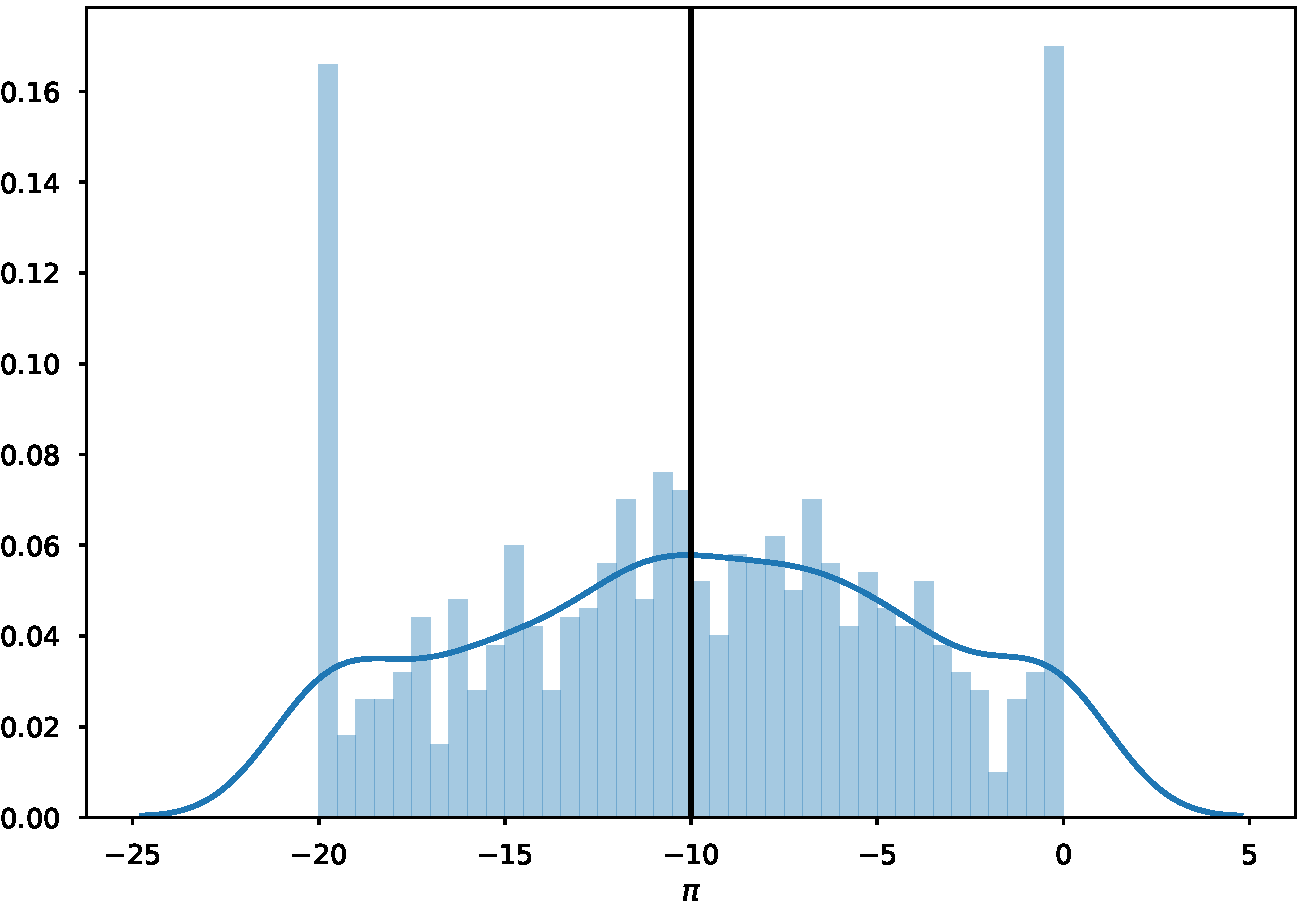
\includegraphics[width=\textwidth, height=\textwidth]{pi_est_250_-0_point_4.pdf}
  \end{subfigure}
  \begin{subfigure}[t]{.32\textwidth}
    \caption[phi = -0.10]{$\phi = -0.10$}
    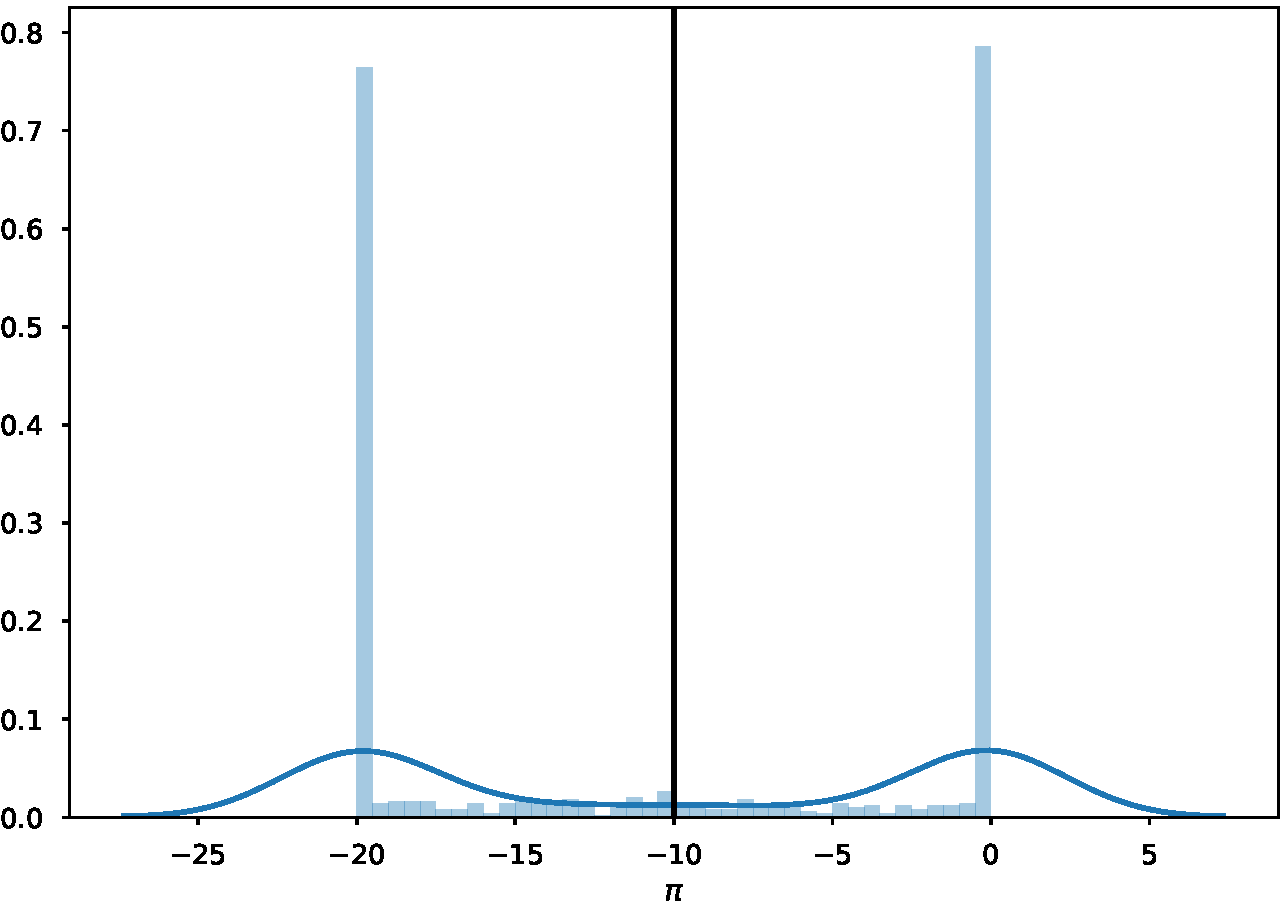
\includegraphics[width=\textwidth, height=\textwidth]{pi_est_250_-0_point_1.pdf}
  \end{subfigure}
  \begin{subfigure}[t]{.32\textwidth}
    \caption[phi = -0.01]{$\phi = -0.01$}
    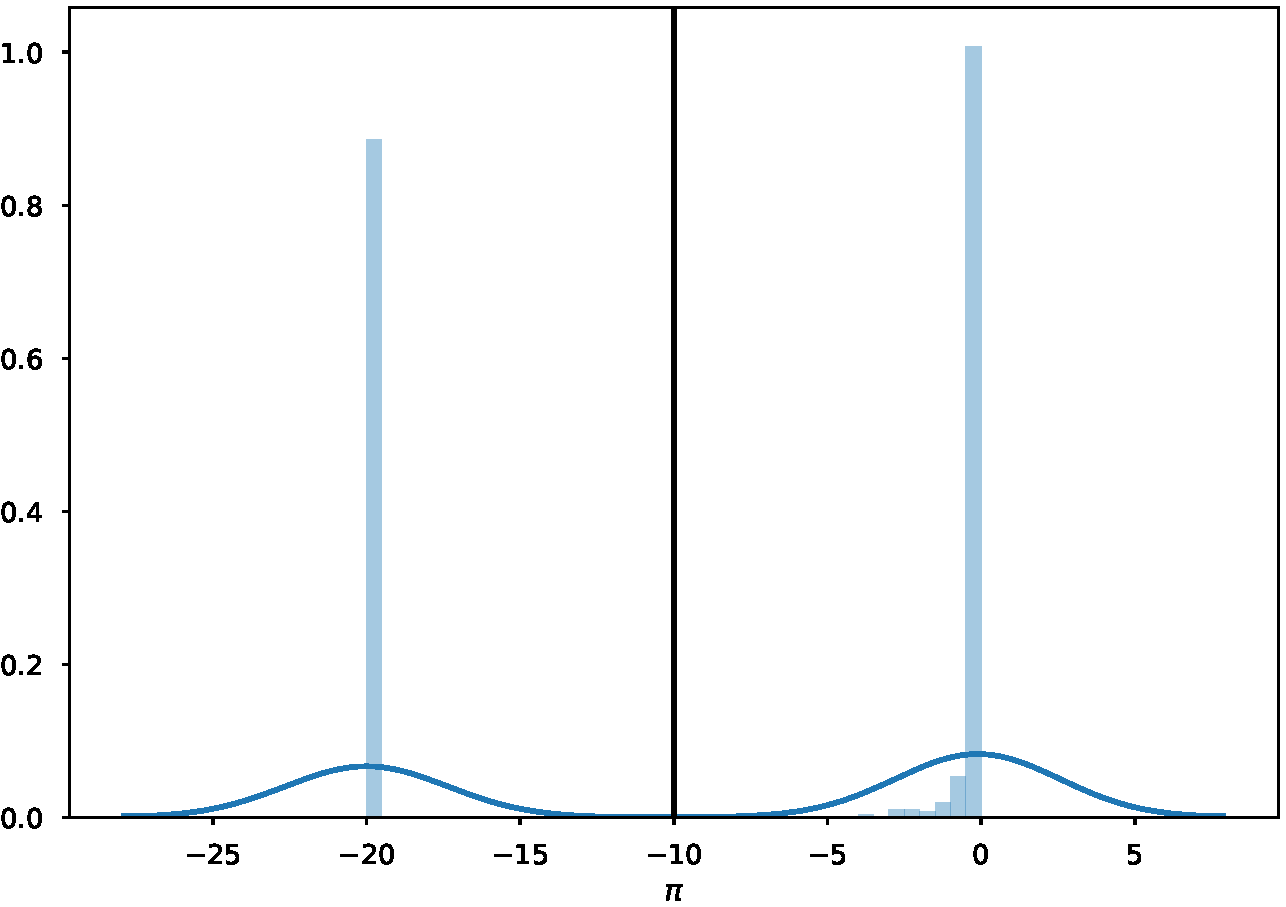
\includegraphics[width=\textwidth, height=\textwidth]{pi_est_250_-0_point_01.pdf}
  \end{subfigure}

\end{figure}


Next, we study the finite-sample size of in the standard QLR test and the proposed conditional QLR test for a joint test for the three structural parameters. The nominal level of the test is \SI{5}{\percent}. The critical value of the standard QLR test is the \SI{95}{\percent} quantile of the chi-square distribution with $3$ degree of freedom. The critical value of the conditional QLR test is obtained by the stimulation-based procedure in \cref{alg:constructing_the_cs}, with \num{1000} simulation repetitions to approximate the quantile of the conditional distribution. The finite-sample size is based on \num{250} simulation repetitions.

The standard test is no longer valid under weak identification because the QLR statistic does not have a chi-square distribution in this case. However, it is not clear whether the standard QLR test under-rejects or over-rejects in finite-sample and how large is the difference from \SI{5}{\percent}. 


\begin{table}[htb]
 
  \centering
  \caption{Finite-Sample Size of the Standard and Proposed Tests}
  \label{tbl:test_performance}

 \sisetup{
  round-mode=places,
  round-precision=2,
 }
 
 \begin{tabularx}{.7\textwidth}{X | S S | S S}
%
  \toprule
  & {Standard} & {Proposed} & {Standard} & {Proposed} \\
  
  \midrule
  $\phi$ & \multicolumn{2}{c}{$T$ = 2,000} & \multicolumn{2}{c}{$T$ = 10,000} \\
  \midrule
  -0.01  & 2.4   & 5.2  & 1.7 & 5.6   \\
  -0.10  & 3.3   & 6.7  & 2.6 & 6.2   \\
  -0.40  & 3.3   & 5.3  & 3.4 & 4.9   \\
  \bottomrule

 \end{tabularx}

\end{table}

Simulation results show that the standard QLR test under-rejects in finite-sample. This is most severe when the identification is weak, i.e., for $\phi=-0.01$, the rejection rate is \SI{2.4}{\percent} and \SI{1.7}{\percent} for the two sample sizes considered, for a \SI{5}{\percent} test. The implication is that the confidence set obtained by inverting the standard test could be much larger than necessary. The conditional QLR test is much less conservative than the standard test. For the two sample sizes considered, the finite-sample reject rate ranges from \SI{4.9}{\percent} to \SI{6.7}{\percent} for a \SI{5}{\percent} test. 

\section{Data and Empirical Results}\label{sec:empirical}

For the empirical application, we use the daily return on the S\&P 500 for $r_{t+1}$ and the associated realized volatility computed with high-frequency data for $\sigma^2_{t+1}$. The data is obtained from SPY (SPDR S\&P 500 ETF Trust), an exchange-traded fund that mimics the S\&P 500. This gives us a market index whose risk is not easily diversifiable and can be used to estimate the prices of risk that investors face in practice. We use the procedure \textcite{sangrey2018jumps} develops to estimate the integrated total volatility, the instantaneous expectation of the price variance. This measure reduces to the integrated diffusion volatility if prices have continuous paths and it works well in the presence of market microstructure noise.

Since SPY is one of the most liquid assets traded, we can choose the frequency at which we sample the underlying price. To balance market-microstructure noise, computational cost, and efficiency of the resultant estimators, we sample at the \num{1} second frequency. The data starts in 2003 and ends in September 2017. Since the asset is only traded during business hours, this leads to \num{3713} days of data with an average of approximately \num{24000} observations per day. We compute $r_{t+1}$ as the daily return from the open to the close of the market, the interval over which we can estimate the volatility. This avoids specifying the relationship between overnight and intra-day returns. We preprocess the data using the pre-averaging approach as in \textcites{podolskij2009bipower, aitsahalia2012testing}. 

%I do not see this is necessary to provide these details. This procedure is known not to affect the consistency of the estimation procedure. The basic idea is rather simple. We average the price over a small interval to remove the noise. If we pick the rates at which we shrink the interval appropriately and thereby balance smoothing away the noise and allowing the volatility to vary intraday, the estimators are consistent.

\begin{figure}[htb]

  \centering
  \caption{S\&P 500 Volatility and Log-Return}


  \begin{subfigure}[t]{.54\textwidth}
    \label{risk_fig:spy_dynamics}
    \caption{Time Series}
    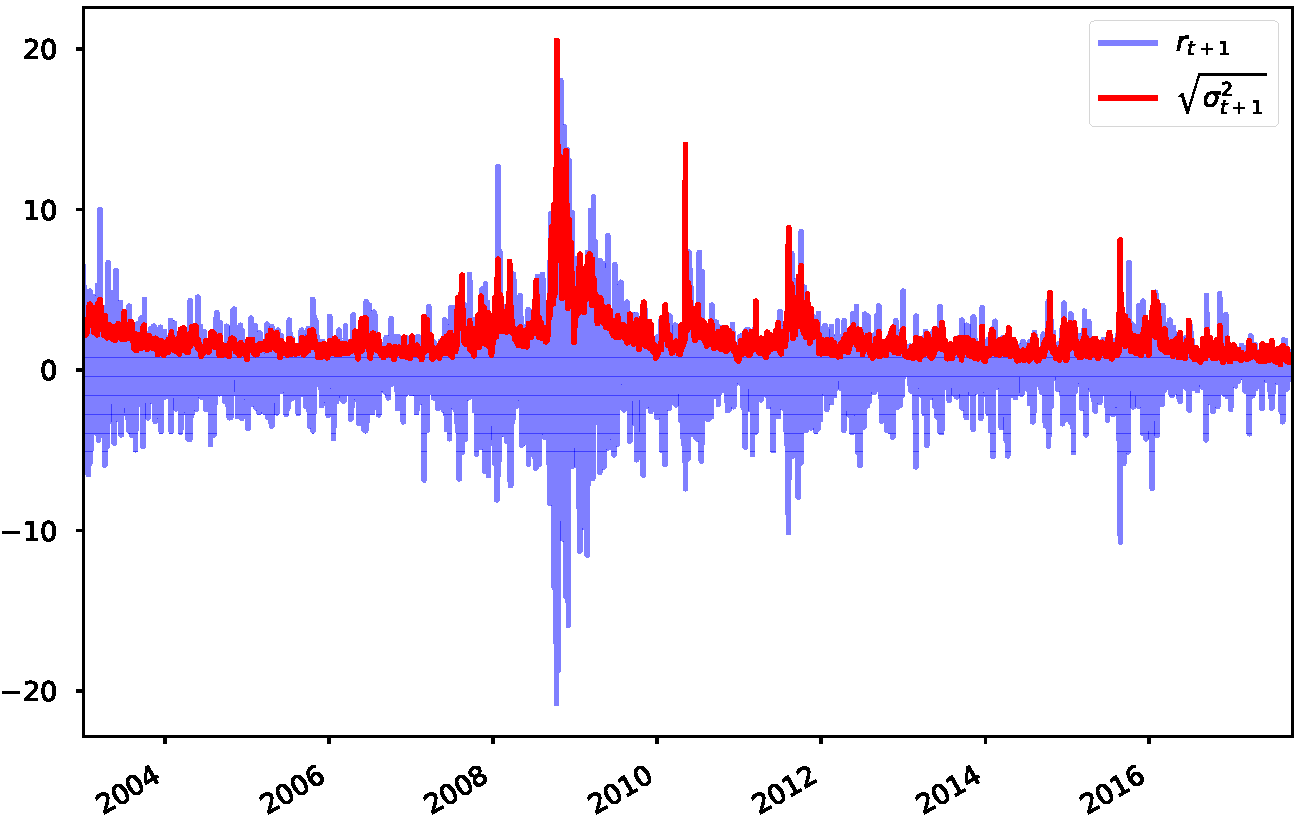
\includegraphics[width=\textwidth, height=.81\textwidth]{time_series.pdf}
  \end{subfigure}%
%
  \hfill
%
  \begin{subfigure}[t]{.44\textwidth}
    \label{risk_fig:spy_static}
    \caption{Joint Distribution}
    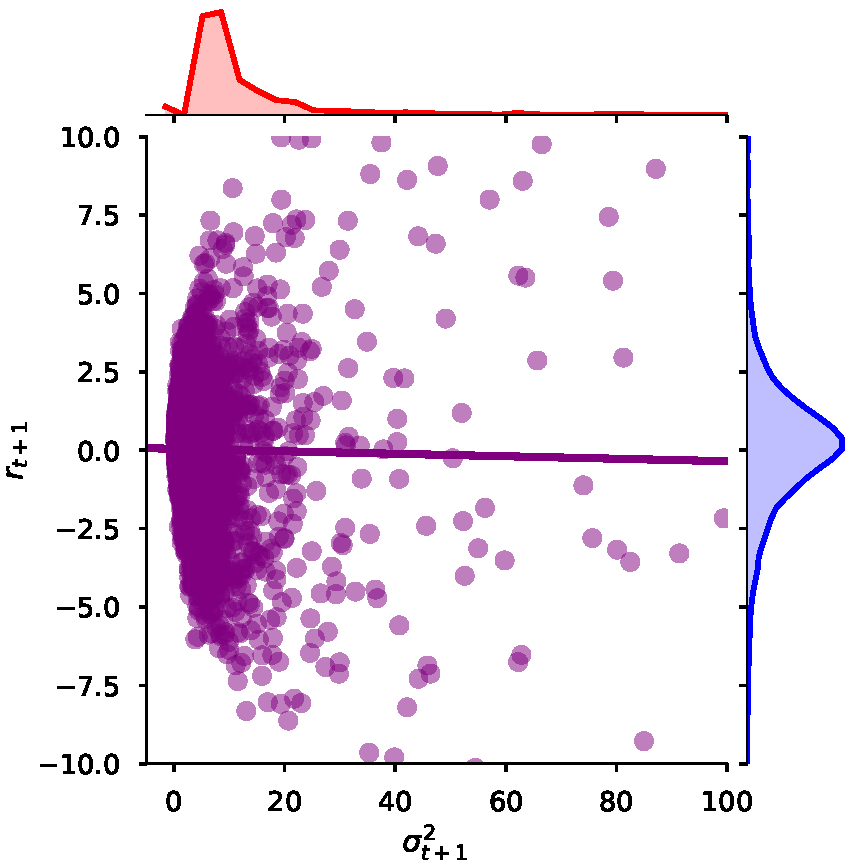
\includegraphics[width=\textwidth, height=\textwidth]{joint_dist.pdf}
  \end{subfigure}
\end{figure}


To see how the data move over time, we plot their time series in  \cref{risk_fig:spy_dynamics}.  We also plot the joint unconditional distribution in \cref{risk_fig:spy_static} to see the static relationship between the two series. The volatility has a long-right tail, a typical gamma-type distribution. The returns has a bell-shaped distribution. They are slightly negatively correlated, as shown by the regression line in the joint plot. This corroborates the work by \textcites{bandi2012timevarying, aitsahalia2013leverage}. We also report a series of summary statistics.

\begin{table}[htb]

  \centering
  \caption{Summary Statistics}
  \label{tbl:summary_stats}


  \sisetup{
   table-align-text-pre=false,
   table-align-text-post=false,
   round-mode=places,
   round-precision=2,
   table-space-text-pre=\lbrack,
   table-space-text-post=\rbrack,
  }

  \begin{tabularx}{.5\textwidth}{X | S S}
    \toprule
    & {$r_{t+1}$} & {$\sigma^2_{t+1}$} \\
    \midrule
      Mean & 0.023421 & 5.621287 \\
      \rowcolor{gray!20}
      Standard Deviation & 2.350165 & 14.458446\\
      Skewness & -0.312 & 12.209 \\
      \rowcolor{gray!20}
      Kurtosis & 10.055 & 240.401 \\
      Correlation & \multicolumn{2}{c}{\num{-0.024379}} \\
    \bottomrule
  \end{tabularx}

\end{table}

We now report the estimates and confidence intervals for the reduced-form parameters $c, \delta$, and $\rho$. The confidence intervals reported here use the Gaussian limiting theory, i.e., the point estimates $\pm 1.96$ standard errors. We first obtain confidence intervals for $\log(c)$ and $\log(c) + \log(\delta)$, and transform them into confidence intervals for $c$ and $\delta$. 

%\footnote{Note, We are not saying that $c$ and $\delta$ are Gaussian distributed, nor are we making any first-order approximations.} I do not see this is helpful in clarification.

%***I do not agree with this statement. For the minimum distance estimate, the other reduced-form paramters play the same role. We have to first estimate all of them and then the simulated critical value is baased on the joint distribution of all the reduced-form paramters. I do not see why c, delta, rho are different from the rest. I think we should report all of them or none of them.We do not report the other reduced-form parameters because they are artifacts of our estimation procedure and are not required to simulate from the model. 

\begin{table}[htb]
  \caption{Reduced-Form Parameters Necessary to Fully Specify the Model} 
  \label{tbl:reduced_form_parameters}

    \centering
    \sisetup{
        detect-mode,
        tight-spacing           = true,
        group-digits            = false,
        input-symbols           = {(}{)},
        input-open-uncertainty  = ,
        input-close-uncertainty = ,
        round-mode              = places,
        round-precision         = 2,
        table-align-text-pre    = false,
        table-align-text-post   = false,
        table-alignment         = center,
    }

    \begin{tabularx}{.7\textwidth}{X | S >{{(}} S[table-space-text-pre={(}] <{{,\,}}
      S[table-space-text-pre={\hspace{-1.5cm}}] <{{)}}}
%
    \toprule
    & {Point Estimate} & \multicolumn{2}{c}{\SI{95}{\percent} Confidence Interval} \\
    \midrule
    $c$     & 6.0678 & 3.47006  & 10.6103 \\
    \rowcolor{gray!20}
    $\delta$  & 0.40814 & 0.2663 & 0.408137969 \\
    $\rho$   & 0.517097 & 0.29481863 & 0.739181 \\
    \bottomrule 
  \end{tabularx}
\end{table}

For confidence intervals of the three structural parameters, we first compute their joint confidence set based on the conditional QLR test and then project it to each of the component. We also plot a joint confidence sets for the two risk prices, after projecting out $\phi$. 


\begin{table}[htb]
  \caption{Structural Parameters} 
  \label{tbl:structural_param_estimates}

  \centering
    \sisetup{
        detect-mode,
        tight-spacing           = true,
        group-digits            = false,
        input-symbols           = {(}{)},
        input-open-uncertainty  = ,
        input-close-uncertainty = ,
        round-mode              = places,
        round-precision         = 2,
        table-align-text-pre    = false,
        table-align-text-post   = false,
        table-alignment         = center,
    }

    \begin{tabularx}{.4\textwidth}{X | S >{{(}} S[table-space-text-pre={(}] <{{,\,}}
      S[table-space-text-pre={\hspace{-1.5cm}}] <{{)}}}
%
    \toprule
    & \multicolumn{2}{c}{\SI{95}{\percent} Confidence Interval} \\
    \midrule
    $\phi$   & -0.20 & -0.10    \\
    \rowcolor{gray!20}
    $\pi$    & -0.02778 & 0.00   \\
    $\kappa$   & 0.333 & 0.3778  \\
    \bottomrule 
  \end{tabularx}
\end{table}

\begin{figure}[htb]
	
	\centering
	\caption{Confidence Set for Risk Prices}
	\label{fig:confidence_region}
	
	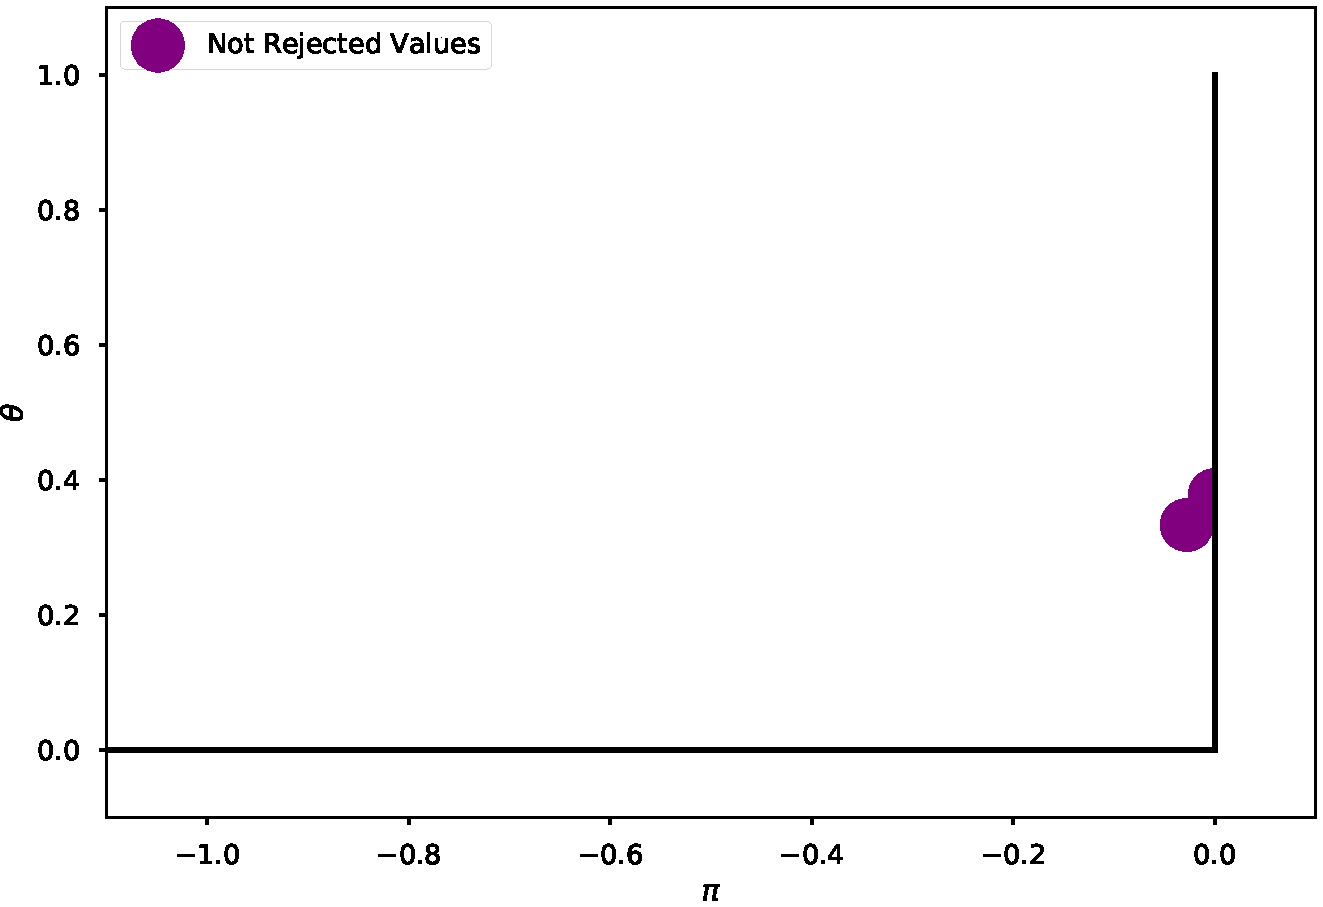
\includegraphics[width=.5\textwidth]{confidence_region_2.pdf}
\end{figure}


The results in \cref{tbl:structural_param_estimates} and \cref{fig:confidence_region} have a few notable features. First, we can reject the null hypothesis $\phi = 0$ at the \SI{5}{\percent} level. We cannot, however, reject the null hypothesis $\pi = 0$. Although the projection procedure leads to conservative subvector confidence sets whose coverage could be larger than \SI{95}{\percent}, the confidence set in \cref{fig:confidence_region} appear to be quite informative. The risk price associated with the market return lies in $(0.33, 0.38)$ with at least \SI{95}{\percent} probability. The volatility risk price is quite small in magnitude, lying in $(-0.03, 0.00)$ with at least \SI{95}{\percent} probability. The point estimates for $\phi, \pi$, and $\kappa$ reported by \textcite{han2018leverage} lie outside our confidence intervals for each of the parameters. They calibrate $\pi = -10$ and then estimate the remaining parameters. This calibrated value of $\pi$ is quite far from its robust confidence interval we construct.

% We're both using data on the S&P 500. We are processing the data differently, but if you  actually want to believe our estimates you have to believe our data processing is reasonable. 
%We use a different data set and process the data differently from those in Han2018. Is this comparision still meaningful? 

%I do not see the following discussion provides more informaiton than their calibraiton is bad, which is already stated above. Also, we do not provide an estimate. Conversely, our estimates do not lie outside their confidence intervals. Even though our estimation procedure for the parameters individually is conservative, as induced by the projection above, our estimates are still more precise in practice. This difference is likely a result of our estimation procedure more effectively using the information about the various parameters jointly, which their partially calibrated model is incapable of doing.

%The main issue with the confidence intervals in \cref{tbl:structural_param_estimates} is that they are conservative because we go from joint inference to sub-vector inference by using an inherently conservative projection-based procedure. Plots of confidence set in three dimensions are not particularly easy to understand, and so we 

%We do impose that kappa is greater than 0. 

%The set is on pi and kappa. We did not impose any constraints on kappa. It is worth noting that except for $\pi < 0$, the constraints on the possible values of the parameters do not bind in practice. Also, as the conditional densities are likely not Gaussian, there is no reason to assume that the confidence sets should be elliptical, and even though the projection procedure is conservative, our confidence set is still quite small. We do not appear to be losing much precision.



\section{Conclusion}\label{sec:risk_conclusion}


In structural stochastic volatility models as the one developed here, changes in the volatility affect returns through two channels. On the one hand, investors are willing to tolerate high volatility to get high expected returns as measured by the price of market return risk. On the other hand, investors are directly averse to changes in future volatility, as measured by the price of volatility risk. \Textcite{han2018leverage} shows how to disentangle these two channels by exploiting information arising from the leverage effect in an exponentially-affine pricing model. However, standard inference for this structural model is invalid because the volatility risk price is only weakly identified when the leverage effect is mild. This paper propose an identification robust inference procedure that provides reliable confidence sets for the risk prices regardless of the magnitude of the leverage effect. We take this procedure to the data on the S\&P 500. The robust inference procedure provides reliable yet informative confidence intervals for the risk prices associated with the market return and the volatility. 




